\documentclass[class=jsarticle, crop=false, dvipdfmx, fleqn]{standalone}
\input{/Users/User/Documents/University/report_template/preamble/preamble}
\begin{document}

\section*{宿題1}

05-21授業分で配布された三種類のデータで,
入力層・隠れ層1つ・出力層からなるニューラルネットワークを誤差逆伝播法により学習させる。

3種類全てのデータに対し,
学習率は0.10とし,隠れ層のノード数は20とした。
また,更新はバッチ学習で行った。
結果を以下の表\ref{tab:result},図\ref{fig:linear}--\ref{fig:slinear}に示す。


\begin{table}[H]
    \centering
    \caption{結果}
    \begin{tabular}{lrrrrr}
        Data Type & {\#}Data & Epoch & Loss & {\#}Correct & Accuracy \\
        linear & 100 & 100 & 0.4534 & 98 & 0.980 \\
        nonlinear & 100 & 5 & 0.9373 & 74 & 0.740 \\
        slinear & 500 & 30 & 0.3786 & 487 & 0.974
    \end{tabular}
    \label{tab:result}
\end{table}

\begin{figure}[H]
    \centering
    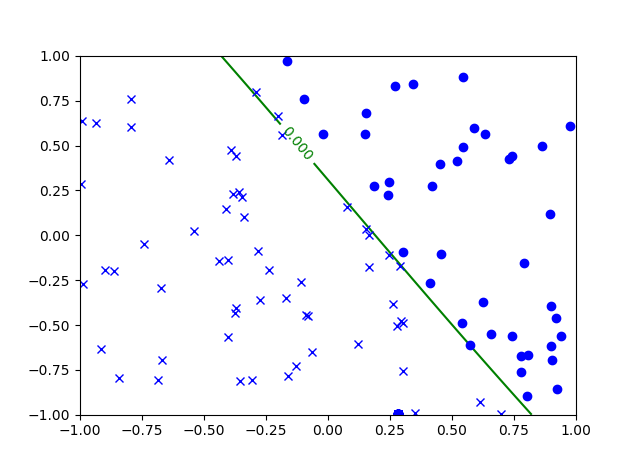
\includegraphics[clip, width=12cm]{../figures/assignment1_1_linear_result}
    \caption{linearデータに対する結果}
    \label{fig:linear}
\end{figure}

\begin{figure}[H]
    \centering
    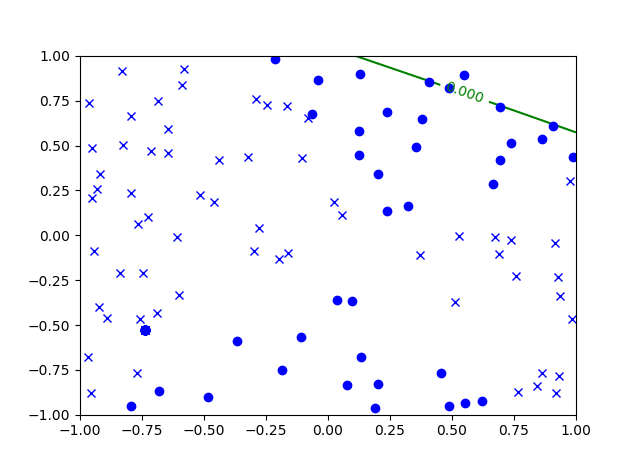
\includegraphics[clip, width=12cm]{../figures/assignment1_1_nonlinear_result}
    \caption{nonlinearデータに対する結果}
    \label{fig:nonlinear}
\end{figure}

\begin{figure}[H]
    \centering
    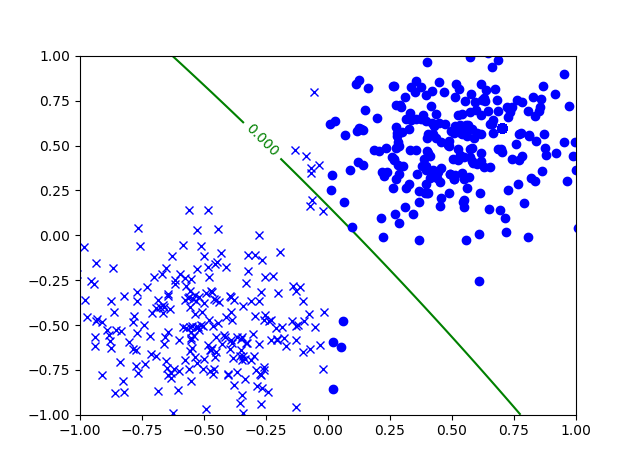
\includegraphics[clip, width=12cm]{../figures/assignment1_1_slinear_result}
    \caption{slinearデータに対する結果}
    \label{fig:slinear}
\end{figure}

\clearpage

プログラムはページ\ref{listing:assignment1}のListing \ref{listing:assignment1}に示した。
また,プログラム中で呼び出している\texttt{neural\_network}モジュールは,
\ref{listing:neural_network}のListing \ref{listing:neural_network}に示した。
以下にまず,\texttt{neural\_network}モジュールの関数とクラスの説明を示す。
なお,このモジュールは宿題3でも用いる。

\begin{itemize}
    \item identity\_function \\
        恒等関数
    \item deriv\_identity\_function \\
        恒等関数の微分
    \item sigmoid \\
        sigmoid関数
    \item deriv\_sigmoid \\
        sigmoid関数の微分
    \item FC \\
        ニューラルネットワークの1層を表すクラス。
        入出力のサイズと活性化関数及びその微分の関数を引数に取る。
        重み・バイアスの他に,それらの勾配,順伝搬時の活性化前の値,誤差なども属性として持つ。
        また,誤差逆伝搬と勾配を計算するメソッドを持つ。
    \item Model \\
        層の構成を引数に取る,モデルを表すクラス。
        全体に対し誤差逆伝搬とパラメータの更新を行うメソッドを持つ。
\end{itemize}

また,以下にassignment1.pyの各関数の説明を示す。

\begin{itemize}
    \item load\_data \\
        .matファイルからデータを読み込む関数
    \item compute\_loss \\
        実値と予測値から損失を計算する関数
    \item plot \\
        境界と点群をプロットする関数
    \item train \\
        ニューラルネットワークのモデルの最適なパラメータを,
        勾配降下法と誤差逆伝搬法によって求める関数
    \item main \\
        実行時の処理をまとめた関数
\end{itemize}


\end{document}
